%%% AgriHome Vision Console — Architectural Design Specification
%%% Structure aligned with CSE 4316 / UTA senior design template

\documentclass[11pt,letterpaper]{article}
\usepackage[margin=1.0in]{geometry}
\usepackage[T1]{fontenc}
\usepackage[bitstream-charter]{mathdesign}
\usepackage[utf8]{inputenc}
\usepackage{amsmath}
\usepackage{array}
\usepackage{xcolor}
\usepackage{hyphenat}
\usepackage{graphicx}
\usepackage{float}
\usepackage{sectsty}
\usepackage[compact]{titlesec}
\usepackage[tablegrid]{vhistory}
\usepackage{pbox}
\usepackage[titles]{tocloft}
\cftsetindents{figure}{0em}{4.2em}
\cftsetindents{table}{0em}{4.2em}
\usepackage[hidelinks]{hyperref}
\usepackage{tikz}
\usetikzlibrary{shapes.geometric,arrows.meta,positioning,fit,backgrounds,calc}

\graphicspath{{images/}}

\allsectionsfont{\color{accentcolor}\scshape\selectfont}

%%% Definitions
\definecolor{accentcolor}{rgb}{0.0,0.0,0.5}
\definecolor{leafgreen}{RGB}{61,159,108}
\newcommand{\teamname}{Agrihome}
\newcommand{\coursename}{CSE 4316: Senior Design I}
\newcommand{\semester}{Spring 2026}
\newcommand{\docname}{Architectural Design Specification}
\newcommand{\department}{Department of Computer Science \& Engineering}
\newcommand{\university}{The University of Texas at Arlington}
% Roster sorted alphabetically by family name
\newcommand{\authors}{%
  GOVINDA AWASTHI\\
  LAXMAN BHUSHAL\\
  THUC DANG\\
  SAGAR KHADKA\\
  MUHAMMAD SAAD MEMON\\
  ALEX TABLIZO\\
  NATHAN NGUYEN TRAN}

%%% Headers and footers
\usepackage{fancyhdr}
\pagestyle{fancy}
\usepackage{lastpage}
\lhead{}
\chead{}
\rhead{}
\lfoot{\footnotesize \teamname\ - \semester}
\cfoot{}
\rfoot{\footnotesize page \thepage\ of \pageref{LastPage}}
\renewcommand{\headrulewidth}{0.0pt}
\renewcommand{\footrulewidth}{0.4pt}

\usepackage[runin]{abstract}
\abslabeldelim{\quad}
\setlength{\abstitleskip}{-10pt}
\renewcommand{\abstractname}{}
\renewcommand{\abstracttextfont}{\color{accentcolor} \small \slshape}

\begin{document}

%%% Cover sheet
{\centering \huge \color{accentcolor} \scshape \textbf{\department \\ \university} \par}
\vspace{0.65in}
{\centering \huge \color{accentcolor} \scshape \textbf{\docname \\ \coursename \\ \semester} \par}
\vspace{0.4in}
\begin{center}
	
\includegraphics[width=0.52\textwidth]{agrihome-logo}\\[0.55em]
	{\small\slshape AgriHome project logo: leaf and camera lens motif for vision-based agricultural monitoring.}
\end{center}
\vspace{0.45in}
{\centering \huge \color{accentcolor} \scshape \textbf{\teamname} \par}
\vspace{0.4in}
{\centering \large \scshape \textbf{\authors} \par}
\newpage

\begin{versionhistory}
	\vhEntry{0.1}{03.04.2026}{Team}{Document created; initial architecture draft}
	\vhEntry{1.0}{03.04.2026}{Team}{Layered overview, figures, PDF verified}
	\vhEntry{1.1}{03.04.2026}{Team}{Raised system-level abstraction in overview sections}
	\vhEntry{2.0}{03.04.2026}{GA, LB, TD, SK, MSM, AT, NNT}{Restructure to CSE 4316 ADS format; subsystems, interfaces; team roster}
\end{versionhistory}
\newpage

\setcounter{tocdepth}{3}
\tableofcontents
\newpage

\listoffigures
\listoftables
\newpage

\section{Introduction}
\subsection{Purpose}

The \textbf{AgriHome Vision Console} is a web-based monitoring and decision-support product for controlled-environment agriculture and laboratory plant studies. Operators and researchers use it to observe tray-level imagery, track individual plants, review automated health assessments, organize trays into logical \textbf{meshes}, manage image-capture schedules, and operate \textbf{Raspberry~Pi / Klipper} edge capture devices. This \textbf{Architectural Design Specification (ADS)} records how the product is decomposed into layers and subsystems, how data moves among them, and which interfaces connect internal components to each other and to external partners.

This document is a companion to the team's \textbf{System Requirements Specification (SRS)} for the same project.\cite{srs} The SRS states \emph{what} the system must do for customers (for example, plant health presentation, automatic capture, environmental data, dashboards, authentication, and secure storage). This ADS states \emph{how} those responsibilities are allocated to software structure: presentation, application orchestration, processing (vision adapters, edge disease hook, schedule runner), persistent data, and hardware edge capture.

\subsection{Scope}

\textbf{In scope} for this ADS are: the logical five-layer architecture (presentation, application, processing, data, hardware); subsystem names, assumptions, responsibilities, and interface summaries; major data flows from user or edge-agent action to storage; identification of optional processing and search backends; Raspberry~Pi / Klipper edge integration at the architectural level; and deployment context at the level of application, database, object storage, and bench devices.\cite{edgeops}

\textbf{Out of scope} are: user-interface visual design mockups beyond structural responsibilities; exhaustive REST field specifications (see engineering docs); source file paths and build commands; formal threat models (see edge security notes); and training procedures for ML models.

\subsection{System summary}

AgriHome addresses limitations of ad hoc spreadsheets, disconnected camera feeds, and manual record-keeping by providing a \textbf{single console} that ties together:

\begin{itemize}
  \item \textbf{Identity and access} — authenticated users interact only with their permitted trays, plants, and meshes; edge devices authenticate with hashed device API keys.
  \item \textbf{Observation} — latest captures, charts, and monitoring history support plant status display, historical data, and dashboard-style summaries.
  \item \textbf{Edge capture} — Raspberry~Pi devices with Agri-Home/klipper (\texttt{fswebcam} via \texttt{save\_image.sh}) auto-provision, heartbeat, and deliver imagery via Take Picture (primary agent capture; optional HTTP streamer still) and scheduled multi-pose capture.\cite{klipper}
  \item \textbf{Interpretation} — health reports and optional model-backed inference (including post-ingest disease analysis) enrich raw imagery where configured.
  \item \textbf{Planning} — schedules express when captures should occur, including destination \texttt{raspberry-pi-edge}.
  \item \textbf{Persistence} — relational storage holds authoritative domain and edge state; object storage holds images referenced from that state.
\end{itemize}

The reference implementation uses a modern full-stack web platform (browser and installable PWA client, server-hosted application, PostgreSQL, file storage, Firebase Authentication, optional HTTP-based inference services, and Python \texttt{agrihome\_agent} on the Pi). The architecture in this document is described so that those technologies could be substituted behind the same layer boundaries where a future maintainer requires it.

\subsection{Document organization}

Section~2 presents the \textbf{project overview} and describes the five primary layers. Section~3 gives a \textbf{system description} with a consolidated subsystem-and-data-flow view. Sections~4--8 document \textbf{data}, \textbf{presentation}, \textbf{application}, \textbf{processing}, and \textbf{hardware} layer subsystems respectively, each with assumptions, responsibilities, and interface tables. The \textbf{References} section lists external citations and the companion SRS.

\newpage

\section{Project Overview}
\label{sec:overview}

The AgriHome Vision Console is designed using a \textbf{layered architecture}. Each layer has a distinct role; layers interact through well-defined interfaces (HTTP APIs between client and server, device-key APIs to edge agents, internal service calls within the server, SQL and file I/O toward stores, optional outbound calls to inference services, and optional HTTP still pulls to LAN streamers). This separation improves modularity, testability, and the ability to scale or replace one concern (for example, swapping a vision provider or webcam path) without rewriting unrelated areas.

The system comprises \textbf{five primary layers}:

\begin{enumerate}
  \item \textbf{Presentation Layer} — user-facing experience in the browser or PWA: landing and marketing entry, authentication, dashboard, tray and plant views, mesh management, schedules, \textbf{Devices} navigation, tray Raspberry~Pi panel with Take Picture, charts, and uploads.
  \item \textbf{Application Layer} — server-side control: HTTP and GraphQL entry points (including \texttt{/api/raspberry-pi/*} and \texttt{/api/devices/*}), session and device-key verification, validation, routing of work to domain services, coordination of reads and writes to the data layer, invocation of the processing layer when needed, and optional HTTP streamer still fetches.
  \item \textbf{Processing Layer} — computer-vision and analytics \emph{adapters}, plus edge post-ingest hooks and the capture schedule runner: optional services that accept images or features and return structured labels, detections, or scores; schedule runners that enqueue \texttt{capture\_now} work for \texttt{raspberry-pi-edge} destinations.
  \item \textbf{Data Layer} — durable storage: relational database for domain and edge entities (\texttt{edge\_devices}, \texttt{edge\_device\_commands}, \texttt{capture\_pose\_sequences}, \texttt{capture\_poses}, \texttt{capture\_schedules}, \texttt{camera\_captures}, \texttt{plants}, \texttt{prediction\_results}, trays, meshes, reports), and object or file storage for imagery; optional vector index for similarity search when enabled.
  \item \textbf{Hardware Layer} — Raspberry~Pi hosts running Agri-Home/klipper (\texttt{fswebcam} / \texttt{camera-macros/save\_image.sh}), optional LAN HTTP streamer bases, and the \texttt{agrihome\_agent} bridge that registers, heartbeats, captures, and ingests.
\end{enumerate}

\subsection{Presentation layer description}

The Presentation Layer is the primary interface between \textbf{people} and the product. It implements responsive layouts for desktop and mobile, supports installable PWA behavior for field-adjacent use, and communicates with the Application Layer exclusively through HTTPS (including authenticated cookie-based sessions after sign-in).

Users register or sign in, navigate trays and plants, upload photos, trigger or view vision-assisted results, inspect monitoring history, configure schedules, manage meshes, and operate \textbf{edge devices} (list devices, edit Klipper/streamer URL, Take Picture from the tray Raspberry~Pi panel). The layer is responsible for presenting SRS-mandated capabilities such as health status, historical trends, dashboard summaries, and settings-oriented flows at a user-experience level; it does not embed direct database access.

\textbf{Key responsibilities:}
\begin{itemize}
  \item Capture user input (forms, file selection, navigation, Take Picture).
  \item Render charts, tables, imagery, device status, and structured errors clearly.
  \item Invoke application APIs and display responses or structured errors.
  \item Encapsulate client-only concerns (progressive enhancement, local caching of shell assets where applicable).
\end{itemize}

\subsection{Application layer description}

The Application Layer is the \textbf{central coordinator}. It receives every authenticated request from the Presentation Layer, interprets it, enforces authorization tied to the authenticated identity, validates payloads, delegates to domain-oriented modules (tray and plant lifecycle, mesh topology, schedules, monitoring logs, file references, edge device actions), and returns responses.

It also terminates \textbf{device-key} traffic from Raspberry~Pi agents (\texttt{/api/raspberry-pi/register}, heartbeat, ingest, commands, poses, capture-plan) and operator device actions (\texttt{/api/devices}). For Take Picture, this layer primarily queues \texttt{capture\_now} for the agent (\texttt{fswebcam}); when \texttt{klipper\_url} is set it may optionally fetch an HTTP streamer still first. It bridges to the Processing Layer for species/disease classification and schedule-driven capture enqueue.

\textbf{Key responsibilities:}
\begin{itemize}
  \item Expose a stable API surface for the console, edge agents, and future integrators.
  \item Maintain session integrity, ownership rules, and hashed device API keys.
  \item Orchestrate transactions across relational updates and file metadata (including multipart ingest).
  \item Isolate failures in optional backends so core monitoring remains usable when possible.
\end{itemize}

\subsection{Processing layer description}

The Processing Layer performs \textbf{compute-intensive or model-based} work and \textbf{asynchronous capture orchestration} that should not block the interactive UI thread. In AgriHome this includes, when configured, \textbf{species or leaf-level classification}, \textbf{tray-level vision}, the \textbf{edge disease hook} after Pi ingest, and the \textbf{capture schedule runner} that enqueues edge capture commands for destinations marked \texttt{raspberry-pi-edge}.

When no external model is available, the Application Layer may apply \textbf{deterministic or simulated} behavior for development and demonstration; the architecture still treats that path as ``processing'' logically because it produces structured inference output distinct from raw CRUD.

\textbf{Key responsibilities:}
\begin{itemize}
  \item Accept image or feature input in a contract agreed with the application tier.
  \item Run detection, embedding, or classification pipelines as implemented (including post-ingest disease analysis).
  \item Return normalized results (labels, confidence, geometry) to the Application Layer.
  \item Enqueue scheduled edge captures without requiring an operator to be present.
  \item Remain stateless with respect to long-term domain truth; persistence is always via the application and data layers.
\end{itemize}

\subsection{Data layer description}

The Data Layer is the \textbf{authoritative foundation} for AgriHome. The relational store holds entities and relationships that satisfy SRS concepts: plant health records over time, capture references, environmental or monitoring events as modeled, mesh membership, schedules, and Summer~2026 \textbf{edge} tables (\texttt{edge\_devices}, \texttt{edge\_device\_commands}, pose sequences/poses). Object storage holds binary assets (camera frames, user uploads) referenced by identifiers or URLs in the relational model.

Optional components such as a \textbf{vector database} participate in this layer when similarity or embedding search is required; they remain secondary to the relational system of record.

\textbf{Key responsibilities:}
\begin{itemize}
  \item Persist and retrieve structured domain and edge data with consistency expectations documented per operation.
  \item Store and stream large binaries efficiently.
  \item Enforce integrity through schema, constraints, and application-side validation.
  \item Support backup, migration, and operational monitoring consistent with deployment policy.
\end{itemize}

\subsection{Hardware layer description}

The Hardware Layer is the \textbf{physical capture plane}. Raspberry~Pi devices run Agri-Home/klipper with \texttt{fswebcam} and the \texttt{agrihome\_agent}, which auto-provisions into AgriHome, reports online status, and delivers imagery by answering queued commands (primary) or by exposing an optional HTTP streamer that the Application Layer can pull when the Pi is LAN-reachable from the server.

\textbf{Key responsibilities:}
\begin{itemize}
  \item Provide durable device identity and local agent configuration.
  \item Expose JPEG snapshot endpoints for server-side and agent-local capture.
  \item Execute pose-aware multi-angle capture when schedules or operators request it.
  \item Avoid autonomous plant-care actuation; motion fields may be stubbed pending hardware bring-up.
\end{itemize}

\subsection{Layered architecture figure}

Figure~\ref{fig:layer-arch} summarizes the five layers and primary external actors. Companion diagrams in Section~3 refine internal subsystems and data flow.

\begin{figure}[H]
\centering
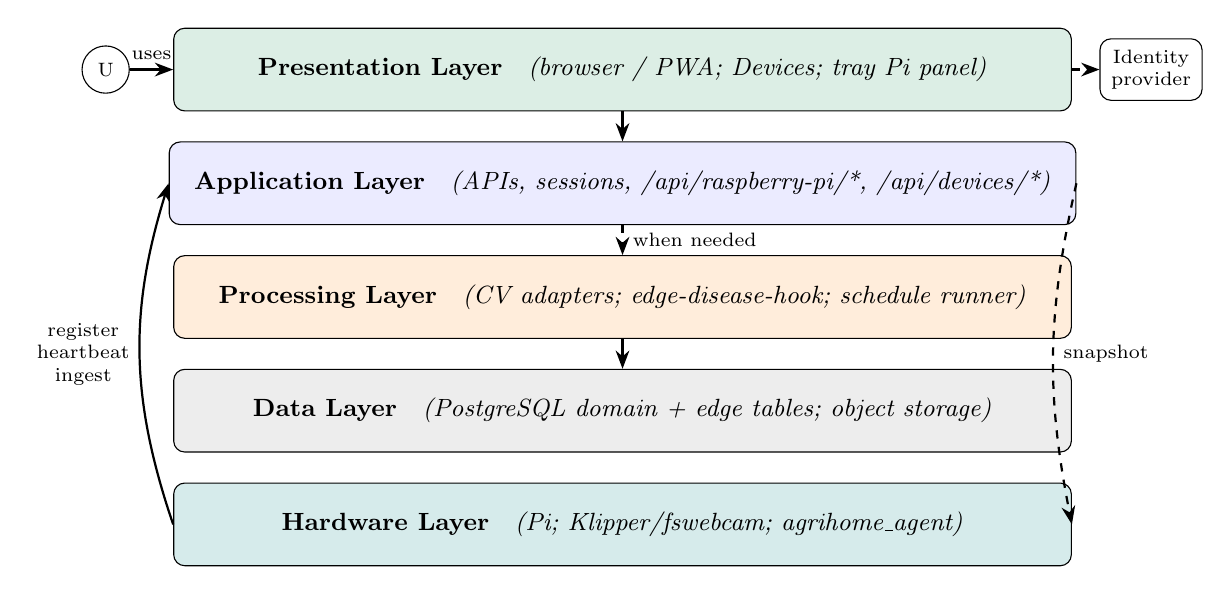
\begin{tikzpicture}[
  font=\small,
  layer/.style={draw, rounded corners, minimum width=11.4cm, minimum height=1.05cm, align=left, inner sep=9pt},
  arr/.style={-{Stealth}, thick},
]
\node[layer, fill=leafgreen!18] (L1) {\textbf{Presentation Layer}\quad\textit{(browser / PWA; Devices; tray Pi panel)}};
\node[layer, below=0.38cm of L1, fill=blue!8] (L2) {\textbf{Application Layer}\quad\textit{(APIs, sessions, /api/raspberry-pi/*, /api/devices/*)}};
\node[layer, below=0.38cm of L2, fill=orange!14] (L3) {\textbf{Processing Layer}\quad\textit{(CV adapters; edge-disease-hook; schedule runner)}};
\node[layer, below=0.38cm of L3, fill=gray!14] (L4) {\textbf{Data Layer}\quad\textit{(PostgreSQL domain + edge tables; object storage)}};
\node[layer, below=0.38cm of L4, fill=teal!16] (L5) {\textbf{Hardware Layer}\quad\textit{(Pi; Klipper/fswebcam; agrihome\_agent)}};

\node[draw, circle, minimum size=0.6cm, left=0.55cm of L1, font=\scriptsize, inner sep=0pt] (u) {U};
\node[draw, rounded corners, font=\scriptsize, right=0.35cm of L1, align=center, inner sep=4pt] (idp) {Identity\\provider};

\draw[arr] (u) -- node[above, font=\scriptsize] {uses} (L1);
\draw[arr, dashed] (L1.east) -- (idp.west);
\draw[arr] (L1.south) -- (L2.north);
\draw[arr, dashed] (L2.south) -- node[right, font=\scriptsize] {when needed} (L3.north);
\draw[arr] (L3.south) -- (L4.north);
\draw[arr, bend left=18] (L5.west) to node[left, font=\scriptsize, align=center] {register\\heartbeat\\ingest} (L2.west);
\draw[arr, dashed, bend right=12] (L2.east) to node[right, font=\scriptsize] {snapshot} (L5.east);
\end{tikzpicture}
\caption{AgriHome Vision Console: five-layer architecture with Pi/Klipper edge trust boundaries.}
\label{fig:layer-arch}
\end{figure}

\subsection{System workflow overview}

A typical end-to-end path begins when a signed-in user opens a \textbf{tray} or \textbf{Devices} view in the Presentation Layer. The client requests data from the Application Layer, which reads the \textbf{Data Layer} (relational and, when needed, media URLs). For \textbf{Take Picture}, the Application Layer primarily queues a command that \texttt{agrihome\_agent} claims on heartbeat, captures via \texttt{fswebcam}/\texttt{save\_image.sh}, and multipart-ingests; if an optional streamer URL is reachable it may pull a still first. When vision-assisted analysis is configured, the Processing Layer's edge disease hook may classify the capture; results return as structured data and are written to \texttt{prediction\_results} / reports. Scheduled \texttt{raspberry-pi-edge} policies are advanced by the capture schedule runner. Updated state flows back to the Presentation Layer for display.

\newpage

\section{System Description}
\label{sec:systemdesc}

This section provides a consolidated \textbf{subsystem definition} and \textbf{data-flow} narrative for the AgriHome Vision Console, including the Summer~2026 Raspberry~Pi / Klipper edge path. Figure~\ref{fig:subsys-flow} maps major building blocks to the five layers introduced in Section~2. The text following the figure walks through each layer and explains how information moves from user or agent intent to durable storage and back.

\begin{figure}[H]
\centering
\scalebox{0.86}{
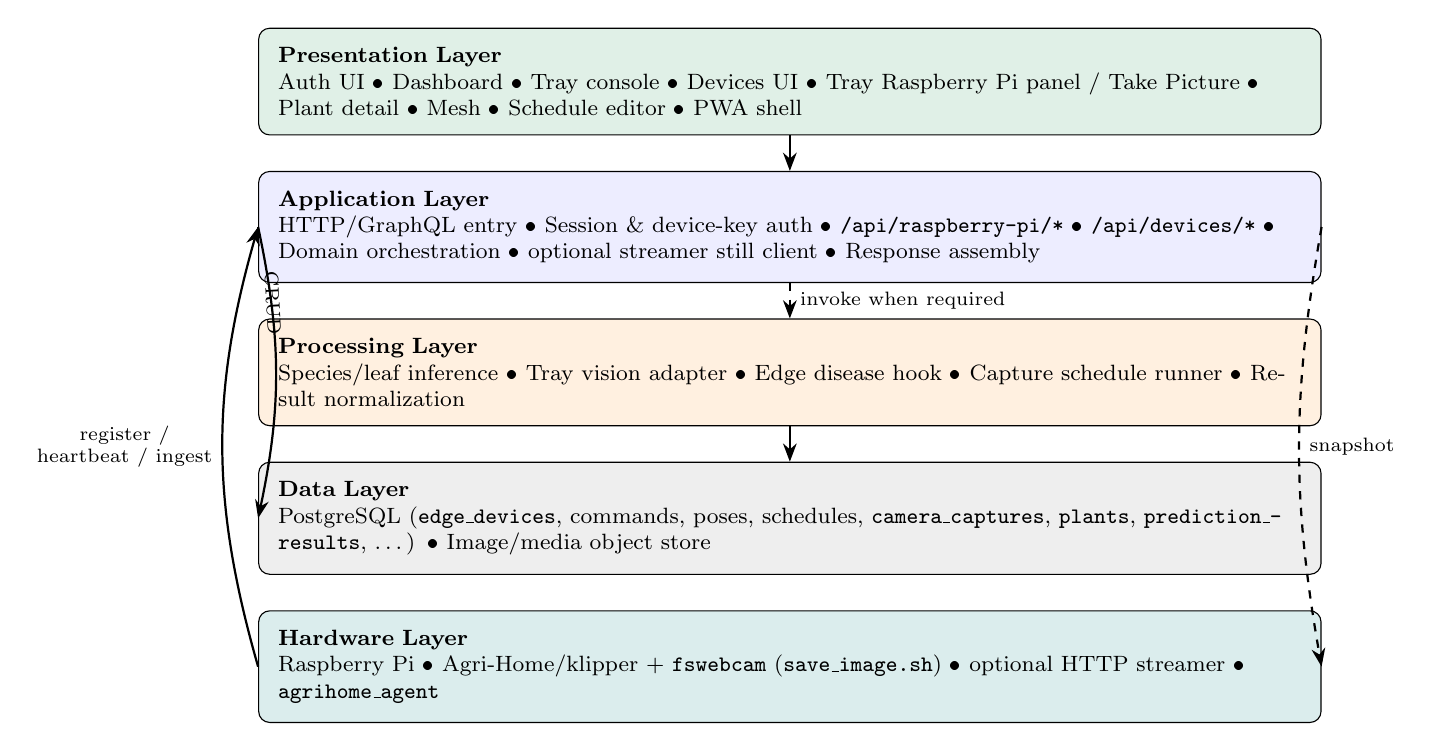
\begin{tikzpicture}[
  font=\footnotesize,
  arr/.style={-{Stealth}, thick},
  band/.style={draw, rounded corners, align=left, inner sep=7pt, text width=13.0cm},
]
\node[band, fill=leafgreen!16] (r1) {
  \textbf{Presentation Layer}\par
  Auth UI \textbullet{} Dashboard \textbullet{} Tray console \textbullet{} Devices UI \textbullet{} Tray Raspberry~Pi panel / Take Picture \textbullet{} Plant detail \textbullet{} Mesh \textbullet{} Schedule editor \textbullet{} PWA shell
};
\node[band, fill=blue!7, below=0.45cm of r1] (r2) {
  \textbf{Application Layer}\par
  HTTP/GraphQL entry \textbullet{} Session \& device-key auth \textbullet{} \texttt{/api/raspberry-pi/*} \textbullet{} \texttt{/api/devices/*} \textbullet{} Domain orchestration \textbullet{} optional streamer still client \textbullet{} Response assembly
};
\node[band, fill=orange!12, below=0.45cm of r2] (r3) {
  \textbf{Processing Layer}\par
  Species/leaf inference \textbullet{} Tray vision adapter \textbullet{} Edge disease hook \textbullet{} Capture schedule runner \textbullet{} Result normalization
};
\node[band, fill=gray!13, below=0.45cm of r3] (r4) {
  \textbf{Data Layer}\par
  PostgreSQL (\texttt{edge\_devices}, commands, poses, schedules, \texttt{camera\_captures}, \texttt{plants}, \texttt{prediction\_results}, \ldots) \textbullet{} Image/media object store
};
\node[band, fill=teal!14, below=0.45cm of r4] (r5) {
  \textbf{Hardware Layer}\par
  Raspberry~Pi \textbullet{} Agri-Home/klipper + \texttt{fswebcam} (\texttt{save\_image.sh}) \textbullet{} optional HTTP streamer \textbullet{} \texttt{agrihome\_agent}
};
\draw[arr] (r1.south) -- (r2.north);
\draw[arr, dashed] (r2.south) -- node[right, font=\scriptsize] {invoke when required} (r3.north);
\draw[arr] (r3.south) -- (r4.north);
\draw[arr, bend left=12] (r2.west) to node[left, font=\scriptsize, sloped, pos=0.4] {CRUD} (r4.west);
\draw[arr, bend left=16] (r5.west) to node[left, font=\scriptsize, align=center] {register /\\heartbeat / ingest} (r2.west);
\draw[arr, dashed, bend right=10] (r2.east) to node[right, font=\scriptsize] {snapshot} (r5.east);
\end{tikzpicture}
}
\caption{Subsystem definitions and primary data flow (edge hardware talks to the application layer; application also reads/writes the data layer directly for most CRUD paths).}
\label{fig:subsys-flow}
\end{figure}

\subsection{Presentation layer composition}

The Presentation Layer is organized around \textbf{workspaces} that match operator mental models. \textbf{Authentication and registration} establish identity and tie the browser to a server session. The \textbf{dashboard} summarizes tray health and recent activity. The \textbf{tray console} shows imagery, monitoring charts, and plant rows for a single tray, including a \textbf{Raspberry~Pi panel} with Take Picture, device link, and Klipper/streamer URL edit. The \textbf{Devices} view lists provisioned edge devices (serial, status, last heartbeat, linked tray). \textbf{Plant detail} focuses on one organism. \textbf{Mesh views} aggregate trays. The \textbf{schedule editor} binds capture policy to trays or meshes, including \texttt{raspberry-pi-edge} destinations. The \textbf{PWA shell} supplies offline-friendly installation where supported.

User gestures in these areas become HTTPS requests to the Application Layer; no presentation component queries the database directly.

\subsection{Application layer composition}

The Application Layer terminates TLS, verifies cookies/tokens or \textbf{device API keys}, and maps the caller to an account or device context. \textbf{Validation} rejects malformed payloads before any side effect. \textbf{Domain orchestration} implements use cases: plant/tray CRUD, meshes, schedules, monitoring, edge register/heartbeat/ingest, operator device actions (\texttt{capture}, \texttt{linkTray}, \texttt{revoke}, \texttt{rotateKey}, \texttt{updateKlipperUrl}), and optional HTTP streamer still attempts. When a use case requires inference, the same layer forwards work to the Processing Layer and merges outcomes into domain writes. \textbf{Response assembly} maps internal results to JSON or GraphQL shapes consumed by the UI or agent.

\subsection{Processing layer composition}

The Processing Layer exposes inference contracts and asynchronous capture helpers. A \textbf{species or leaf adapter} may classify a single-plant photo. A \textbf{tray vision adapter} may estimate plant count or regions. The \textbf{edge disease hook} optionally classifies captures after Pi ingest. The \textbf{capture schedule runner} evaluates due schedules with destination \texttt{raspberry-pi-edge} and enqueues \texttt{capture\_now} (optionally with \texttt{runPoses}). \textbf{Result normalization} keeps bounding boxes, labels, and scores consistent before persistence.

\subsection{Data layer composition}

The Data Layer splits \textbf{transactional} concerns from \textbf{bulk media}. Write coordination sequences inserts so relational rows and file metadata stay aligned. Integrity constraints guard keys and ownership. Query execution runs against \textbf{PostgreSQL}, which holds trays, plants, meshes, schedules, monitoring events, predictions, reports, and edge tables (\texttt{edge\_devices}, \texttt{edge\_device\_commands}, \texttt{capture\_pose\_sequences}, \texttt{capture\_poses}, \texttt{capture\_schedules}, \texttt{camera\_captures}). The \textbf{object store} retains images; the relational model stores pointers.

\subsection{Hardware layer composition}

The Hardware Layer is the bench capture plane: a \textbf{Raspberry~Pi} host, \textbf{Agri-Home/klipper} with \texttt{fswebcam}, optional HTTP streamer, and \textbf{\texttt{agrihome\_agent}}. Agents register and heartbeat; operators trigger Take Picture; schedules drive multi-pose walks. Primary capture is agent + \texttt{fswebcam}; optional server-side stills use a LAN-reachable \texttt{klipper\_url}.

\subsection{End-to-end data flow summary}

The data flow begins when a user interacts with the Presentation Layer or when an edge agent heartbeats. Requests pass to the Application Layer, which authorizes and validates them. Ordinary reads query the Data Layer. Take Picture primarily queues a command claimed by the Hardware Layer agent (\texttt{fswebcam}); it may optionally pull JPEG bytes from an HTTP streamer. Vision-assisted actions call the Processing Layer, then commit structured outputs through the Data Layer. Responses propagate back to the Presentation Layer (or agent) for rendering or further capture steps.

\newpage

\section{Data Layer Subsystems}
The Data Layer provides durable storage for all AgriHome domain state and media. It is structured into subsystems that mirror the reference senior-design pattern: coordinated writes, integrity checks, query execution, the primary relational database, and dedicated image storage.

\subsection{Write coordination subsystem}

The \textbf{write coordination} subsystem sequences operations that must stay consistent across multiple rows or across database rows and file metadata (for example, creating a plant and linking an uploaded photo). It receives structured write intents from the Application Layer and orders them so partial failures can be detected and reported.

\begin{figure}[H]
\centering
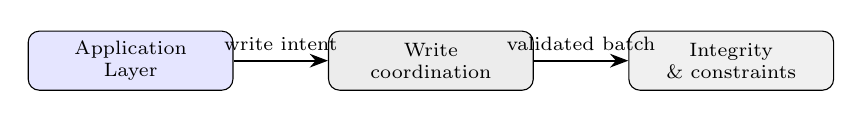
\begin{tikzpicture}[font=\scriptsize, box/.style={draw, rounded corners, align=center, minimum width=2.6cm, minimum height=0.75cm}, arr/.style={-{Stealth}, thick}]
\node[box, fill=blue!10] (app) {Application\\Layer};
\node[box, right=1.2cm of app, fill=gray!15] (wc) {Write\\coordination};
\node[box, right=1.2cm of wc, fill=gray!12] (ic) {Integrity\\\& constraints};
\draw[arr] (app) -- node[above] {write intent} (wc);
\draw[arr] (wc) -- node[above] {validated batch} (ic);
\end{tikzpicture}
\caption{Write coordination subsystem: accepts write intents and forwards them toward integrity checks.}
\label{fig:data-write}
\end{figure}

\subsubsection{Assumptions}
\begin{itemize}
  \item The Application Layer supplies writes in transactional units appropriate to each use case.
  \item Concurrent writers may exist; isolation expectations are defined per operation.
  \item Object storage availability may differ from database availability; coordination must surface errors clearly.
\end{itemize}

\subsubsection{Responsibilities}
\begin{itemize}
  \item Accept batched write intents from domain services.
  \item Order dependent operations (metadata before binary commit or the reverse, per policy).
  \item Expose success/failure to the Application Layer for user-visible error handling.
\end{itemize}

\subsubsection{Subsystem interfaces}
\begin{table}[H]
\centering
\small
\begin{tabular}{|p{0.85cm}|p{3.5cm}|p{3.0cm}|p{3.5cm}|}
\hline
\textbf{ID} & \textbf{Description} & \textbf{Inputs} & \textbf{Outputs} \\
\hline
D-W1 & Application $\rightarrow$ Write coordination & Domain write DTOs & Ordered write plan \\
\hline
D-W2 & Write coordination $\rightarrow$ Integrity & Planned writes & Validation requests \\
\hline
\end{tabular}
\caption{Write coordination subsystem interfaces}
\end{table}

\subsection{Integrity and constraint enforcement subsystem}

This subsystem enforces \textbf{schema rules, referential integrity, and business invariants} before data reaches the query executor. It corresponds to database constraints plus application-level checks that are not expressible as single-column rules.

\begin{figure}[H]
\centering
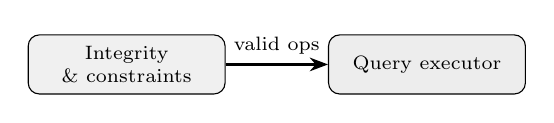
\begin{tikzpicture}[font=\scriptsize, box/.style={draw, rounded corners, align=center, minimum width=2.5cm, minimum height=0.75cm}, arr/.style={-{Stealth}, thick}]
\node[box, fill=gray!12] (ic) {Integrity\\\& constraints};
\node[box, right=1.3cm of ic, fill=gray!14] (qe) {Query executor};
\draw[arr] (ic) -- node[above] {valid ops} (qe);
\end{tikzpicture}
\caption{Integrity subsystem: validates operations before execution.}
\label{fig:data-integrity}
\end{figure}

\subsubsection{Assumptions}
\begin{itemize}
  \item Invalid data may arrive from bugs or malicious clients; all paths must be validated server-side.
  \item Constraint definitions evolve with schema migrations.
\end{itemize}

\subsubsection{Responsibilities}
\begin{itemize}
  \item Reject writes that violate keys, foreign keys, or required fields.
  \item Apply cross-field rules (for example, ownership of a tray by the authenticated account).
  \item Return structured validation failures to the Application Layer.
\end{itemize}

\subsubsection{Subsystem interfaces}
\begin{table}[H]
\centering
\small
\begin{tabular}{|p{0.85cm}|p{3.5cm}|p{3.0cm}|p{3.5cm}|}
\hline
\textbf{ID} & \textbf{Description} & \textbf{Inputs} & \textbf{Outputs} \\
\hline
D-I1 & Write coordination $\rightarrow$ Integrity & Planned writes & Pass/fail + reasons \\
\hline
D-I2 & Integrity $\rightarrow$ Query executor & Validated SQL ops & Executable statements \\
\hline
\end{tabular}
\caption{Integrity and constraint enforcement subsystem interfaces}
\end{table}

\subsection{Query and transaction execution subsystem}

The \textbf{query executor} runs SQL against PostgreSQL: transactional reads, inserts, updates, and deletes issued after validation. It returns rows, counts, or errors to the Application Layer.

\begin{figure}[H]
\centering
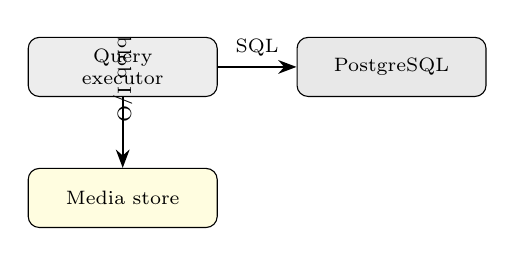
\begin{tikzpicture}[font=\scriptsize, box/.style={draw, rounded corners, align=center, minimum width=2.4cm, minimum height=0.75cm}, arr/.style={-{Stealth}, thick}]
\node[box, fill=gray!14] (qe) {Query\\executor};
\node[box, right=1.0cm of qe, fill=gray!18] (pg) {PostgreSQL};
\node[box, below=0.9cm of qe, fill=yellow!12] (fs) {Media store};
\draw[arr] (qe) -- node[above] {SQL} (pg);
\draw[arr] (qe) -- node[left, font=\scriptsize, sloped] {blob I/O} (fs);
\end{tikzpicture}
\caption{Query executor: issues SQL and coordinates binary I/O with storage.}
\label{fig:data-query}
\end{figure}

\subsubsection{Assumptions}
\begin{itemize}
  \item Connection pooling is managed by the Application Layer infrastructure.
  \item Long-running analytics queries are out of scope for interactive paths.
\end{itemize}

\subsubsection{Responsibilities}
\begin{itemize}
  \item Execute parameterized statements for safety.
  \item Commit or roll back transactions per request scope.
  \item Surface deadlocks and transient errors for retry policy in higher layers.
\end{itemize}

\subsubsection{Subsystem interfaces}
\begin{table}[H]
\centering
\small
\begin{tabular}{|p{0.85cm}|p{3.5cm}|p{3.0cm}|p{3.5cm}|}
\hline
\textbf{ID} & \textbf{Description} & \textbf{Inputs} & \textbf{Outputs} \\
\hline
D-Q1 & Integrity $\rightarrow$ Query executor & Validated ops & Result sets / status \\
\hline
D-Q2 & Query executor $\rightarrow$ PostgreSQL & SQL + params & Rows / ack \\
\hline
D-Q3 & Query executor $\rightarrow$ Media store & Put/get requests & Handles / streams \\
\hline
\end{tabular}
\caption{Query and transaction execution subsystem interfaces}
\end{table}

\subsection{PostgreSQL domain database subsystem}

The \textbf{relational database} is the system of record for trays, plants, meshes, schedules, monitoring events, predictions, reports, and linkage to media. It satisfies SRS needs for structured historical data and dashboard queries.

\begin{figure}[H]
\centering
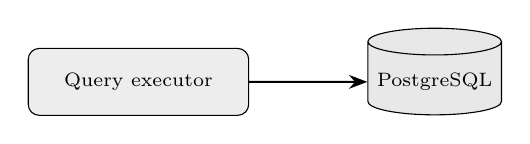
\begin{tikzpicture}[font=\scriptsize, box/.style={draw, rounded corners, align=center, minimum width=2.8cm, minimum height=0.85cm}, arr/.style={-{Stealth}, thick}]
\node[cylinder, shape border rotate=90, aspect=0.2, draw, fill=gray!18, minimum height=1.1cm] (db) {PostgreSQL};
\node[box, left=1.5cm of db, fill=gray!14] (qe) {Query executor};
\draw[arr] (qe) -- (db);
\end{tikzpicture}
\caption{PostgreSQL domain database subsystem.}
\label{fig:data-pg}
\end{figure}

\subsubsection{Assumptions}
\begin{itemize}
  \item Schema is versioned; migrations are applied through controlled processes.
  \item Backup and restore procedures meet institutional RPO/RTO.
\end{itemize}

\subsubsection{Responsibilities}
\begin{itemize}
  \item Persist authoritative entities and relationships.
  \item Support indexed access paths for tray/plant/mesh navigation.
  \item Retain audit-relevant history as required by product policy.
\end{itemize}

\subsubsection{Subsystem interfaces}
\begin{table}[H]
\centering
\small
\begin{tabular}{|p{0.85cm}|p{3.5cm}|p{3.0cm}|p{3.5cm}|}
\hline
\textbf{ID} & \textbf{Description} & \textbf{Inputs} & \textbf{Outputs} \\
\hline
D-P1 & Query executor $\rightarrow$ PostgreSQL & SQL & Tabular results \\
\hline
D-P2 & PostgreSQL $\rightarrow$ Query executor & Internal state & Constraints / errors \\
\hline
\end{tabular}
\caption{PostgreSQL domain database subsystem interfaces}
\end{table}

\subsection{Image and media storage subsystem}

\textbf{Image and media storage} holds camera frames, user uploads, and other large binaries. The Application Layer stores objects and retains stable references in the relational database for use in URLs served back to the Presentation Layer.

\begin{figure}[H]
\centering
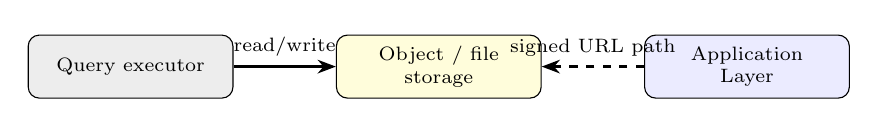
\begin{tikzpicture}[font=\scriptsize, box/.style={draw, rounded corners, align=center, minimum width=2.6cm, minimum height=0.8cm}, arr/.style={-{Stealth}, thick}]
\node[box, fill=yellow!14] (fs) {Object / file\\storage};
\node[box, left=1.3cm of fs, fill=gray!14] (qe) {Query executor};
\node[box, right=1.3cm of fs, fill=blue!8] (app) {Application\\Layer};
\draw[arr] (qe) -- node[above] {read/write} (fs);
\draw[arr, dashed] (app) -- node[above] {signed URL path} (fs);
\end{tikzpicture}
\caption{Image and media storage subsystem and relationship to application reads.}
\label{fig:data-media}
\end{figure}

\subsubsection{Assumptions}
\begin{itemize}
  \item Storage roots are configurable per deployment environment.
  \item Virus scanning or content policy, if required, occurs at integration boundaries.
\end{itemize}

\subsubsection{Responsibilities}
\begin{itemize}
  \item Store and retrieve binaries keyed by application-managed paths or IDs.
  \item Enforce size and type limits cooperatively with validation in the Application Layer.
\end{itemize}

\subsubsection{Subsystem interfaces}
\begin{table}[H]
\centering
\small
\begin{tabular}{|p{0.85cm}|p{3.5cm}|p{3.0cm}|p{3.5cm}|}
\hline
\textbf{ID} & \textbf{Description} & \textbf{Inputs} & \textbf{Outputs} \\
\hline
D-M1 & Query executor $\rightarrow$ Media store & Bytes + path & Ack / handle \\
\hline
D-M2 & Media store $\rightarrow$ Application & Stream requests & File bytes \\
\hline
D-M3 & Application $\rightarrow$ Presentation & Media URL & Rendered imagery \\
\hline
\end{tabular}
\caption{Image and media storage subsystem interfaces}
\end{table}

\newpage

\section{Presentation Layer Subsystems}
The Presentation Layer implements all user-visible behavior described at a high level in the SRS: authentication, dashboards, plant health display, historical views, scheduling, mesh-oriented navigation, and Summer~2026 \textbf{edge device} controls (Devices list, tray Raspberry~Pi panel, Take Picture). Each subsystem below corresponds to a coherent screen family or cross-cutting UI concern.

\subsection{Authentication and session UI subsystem}

This subsystem collects credentials or OAuth flows, exchanges tokens for server sessions, and guards entry to protected routes. It satisfies SRS \textbf{user authentication} expectations at the UX level.

\begin{figure}[H]
\centering
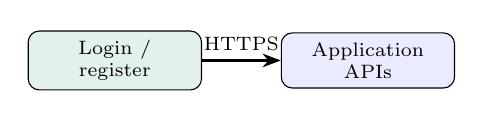
\begin{tikzpicture}[font=\scriptsize, box/.style={draw, rounded corners, align=center, minimum width=2.2cm, minimum height=0.7cm}, arr/.style={-{Stealth}, thick}]
\node[box, fill=leafgreen!15] (login) {Login /\\register};
\node[box, right=1.0cm of login, fill=blue!8] (api) {Application\\APIs};
\draw[arr] (login) -- node[above] {HTTPS} (api);
\end{tikzpicture}
\caption{Authentication UI: user actions become authenticated API calls.}
\label{fig:pres-auth}
\end{figure}

\subsubsection{Assumptions}
\begin{itemize}
  \item Users have network connectivity for initial sign-in.
  \item Identity provider availability matches organizational SLA.
\end{itemize}

\subsubsection{Responsibilities}
\begin{itemize}
  \item Render sign-in, registration, and sign-out affordances.
  \item Hold short-lived client tokens only as required by the chosen identity integration.
  \item Redirect unauthenticated visitors away from protected console routes.
\end{itemize}

\subsubsection{Subsystem interfaces}
\begin{table}[H]
\centering
\small
\begin{tabular}{|p{0.9cm}|p{3.4cm}|p{3.0cm}|p{3.5cm}|}
\hline
\textbf{ID} & \textbf{Description} & \textbf{Inputs} & \textbf{Outputs} \\
\hline
P-A1 & User $\rightarrow$ Auth UI & Credentials / OAuth & Sign-in intent \\
\hline
P-A2 & Auth UI $\rightarrow$ Application & Session exchange requests & HTTP-only session \\
\hline
\end{tabular}
\caption{Authentication and session UI subsystem interfaces}
\end{table}

\subsection{Dashboard and overview subsystem}

The \textbf{dashboard} aggregates tray summaries, recent captures or predictions where available, and entry points into deeper views. It supports SRS \textbf{dashboard interface} and high-level plant status visibility.

\begin{figure}[H]
\centering
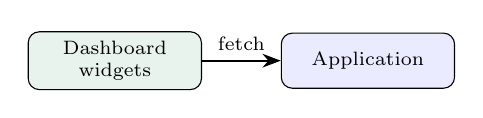
\begin{tikzpicture}[font=\scriptsize, box/.style={draw, rounded corners, align=center, minimum width=2.2cm, minimum height=0.7cm}, arr/.style={-{Stealth}, thick}]
\node[box, fill=leafgreen!12] (dash) {Dashboard\\widgets};
\node[box, right=1.0cm of dash, fill=blue!8] (api) {Application};
\draw[arr] (dash) -- node[above] {fetch} (api);
\end{tikzpicture}
\caption{Dashboard subsystem requests summary aggregates from the application tier.}
\label{fig:pres-dash}
\end{figure}

\subsubsection{Assumptions}
\begin{itemize}
  \item Summary data volume is bounded for interactive load times.
  \item Chart libraries render only on supported browsers.
\end{itemize}

\subsubsection{Responsibilities}
\begin{itemize}
  \item Display tray list and key health indicators.
  \item Link to tray detail, plants, and schedules.
  \item Surface empty and error states clearly.
\end{itemize}

\subsubsection{Subsystem interfaces}
\begin{table}[H]
\centering
\small
\begin{tabular}{|p{0.9cm}|p{3.4cm}|p{3.0cm}|p{3.5cm}|}
\hline
\textbf{ID} & \textbf{Description} & \textbf{Inputs} & \textbf{Outputs} \\
\hline
P-D1 & Dashboard $\rightarrow$ Application & Filter context & Summary DTOs \\
\hline
P-D2 & Application $\rightarrow$ Dashboard & JSON payloads & Rendered charts / lists \\
\hline
\end{tabular}
\caption{Dashboard and overview subsystem interfaces}
\end{table}

\subsection{Tray monitoring console subsystem}

The \textbf{tray console} shows the active tray: latest imagery, monitoring trends, plant thumbnails, events, optional tray-level vision uploads, and the embedded \textbf{Raspberry~Pi panel}. It aligns with \textbf{automatic image capture} presentation and tray-scoped monitoring in the SRS.

\begin{figure}[H]
\centering
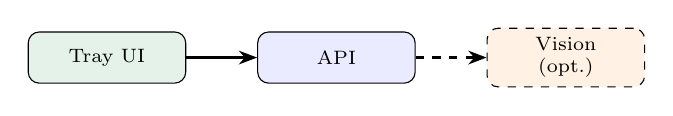
\begin{tikzpicture}[font=\scriptsize, box/.style={draw, rounded corners, align=center, minimum width=2.0cm, minimum height=0.65cm}, arr/.style={-{Stealth}, thick}]
\node[box, fill=leafgreen!14] (ui) {Tray UI};
\node[box, right=0.9cm of ui, fill=blue!8] (api) {API};
\node[box, right=0.9cm of api, fill=orange!10, dashed] (cv) {Vision\\(opt.)};
\draw[arr] (ui) -- (api);
\draw[arr, dashed] (api) -- (cv);
\end{tikzpicture}
\caption{Tray console: drives reads and optional vision requests through the application layer.}
\label{fig:pres-tray}
\end{figure}

\subsubsection{Assumptions}
\begin{itemize}
  \item Each tray identifier maps to authorized user scope.
  \item Large images may be progressively loaded or thumbnailed.
  \item A tray may be linked to zero or one \texttt{edge\_devices} row.
\end{itemize}

\subsubsection{Responsibilities}
\begin{itemize}
  \item Render tray imagery, charts, and plant rows.
  \item Submit tray-scoped uploads or vision jobs as permitted.
  \item Host the Raspberry~Pi panel affordances (link device, Take Picture, Klipper/streamer URL).
  \item Poll or refresh data according to UX policy.
\end{itemize}

\subsubsection{Subsystem interfaces}
\begin{table}[H]
\centering
\small
\begin{tabular}{|p{0.9cm}|p{3.4cm}|p{3.0cm}|p{3.5cm}|}
\hline
\textbf{ID} & \textbf{Description} & \textbf{Inputs} & \textbf{Outputs} \\
\hline
P-T1 & Tray UI $\rightarrow$ Application & Tray ID, actions & Tray detail DTO \\
\hline
P-T2 & Tray UI $\rightarrow$ Application & Image multipart & Vision job result \\
\hline
\end{tabular}
\caption{Tray monitoring console subsystem interfaces}
\end{table}

\subsection{Plant detail and health history subsystem}

\textbf{Plant detail} focuses on a single plant: editable metadata, photo gallery, health reports over time, and scoped monitoring logs. It directly supports SRS \textbf{plant health status} and \textbf{historical data display}.

\begin{figure}[H]
\centering
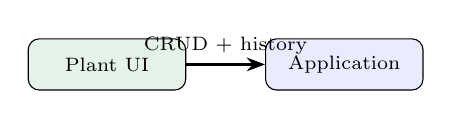
\begin{tikzpicture}[font=\scriptsize, box/.style={draw, rounded corners, align=center, minimum width=2.0cm, minimum height=0.65cm}, arr/.style={-{Stealth}, thick}]
\node[box, fill=leafgreen!14] (p) {Plant UI};
\node[box, right=1.0cm of p, fill=blue!8] (api) {Application};
\draw[arr] (p) -- node[above] {CRUD + history} (api);
\end{tikzpicture}
\caption{Plant detail subsystem: CRUD and reporting views.}
\label{fig:pres-plant}
\end{figure}

\subsubsection{Assumptions}
\begin{itemize}
  \item Users may edit only plants they own or that policy allows.
  \item Report history may be lengthy; pagination or lazy loading applies.
\end{itemize}

\subsubsection{Responsibilities}
\begin{itemize}
  \item Display health timeline and latest findings.
  \item Support photo upload and deletion with confirmation.
  \item Invoke ``add plant from photo'' flows when enabled.
\end{itemize}

\subsubsection{Subsystem interfaces}
\begin{table}[H]
\centering
\small
\begin{tabular}{|p{0.9cm}|p{3.4cm}|p{3.0cm}|p{3.5cm}|}
\hline
\textbf{ID} & \textbf{Description} & \textbf{Inputs} & \textbf{Outputs} \\
\hline
P-P1 & Plant UI $\rightarrow$ Application & Plant ID & Detail + reports \\
\hline
P-P2 & Plant UI $\rightarrow$ Application & Edits / uploads & Updated plant \\
\hline
\end{tabular}
\caption{Plant detail and health history subsystem interfaces}
\end{table}

\subsection{Mesh and topology subsystem}

\textbf{Mesh views} let users group trays for aggregated charts and cross-tray plant listings, supporting experimental layouts described in the SRS's organizational needs without mandating a particular hardware topology.

\begin{figure}[H]
\centering
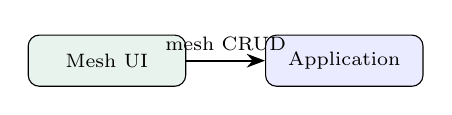
\begin{tikzpicture}[font=\scriptsize, box/.style={draw, rounded corners, align=center, minimum width=2.0cm, minimum height=0.65cm}, arr/.style={-{Stealth}, thick}]
\node[box, fill=leafgreen!12] (m) {Mesh UI};
\node[box, right=1.0cm of m, fill=blue!8] (api) {Application};
\draw[arr] (m) -- node[above] {mesh CRUD} (api);
\end{tikzpicture}
\caption{Mesh subsystem interacts with mesh and member tray aggregates.}
\label{fig:pres-mesh}
\end{figure}

\subsubsection{Assumptions}
\begin{itemize}
  \item Mesh membership changes are infrequent relative to reads.
\end{itemize}

\subsubsection{Responsibilities}
\begin{itemize}
  \item Create and list meshes; show merged monitoring where available.
  \item Navigate from mesh to constituent trays and plants.
\end{itemize}

\subsubsection{Subsystem interfaces}
\begin{table}[H]
\centering
\small
\begin{tabular}{|p{0.9cm}|p{3.4cm}|p{3.0cm}|p{3.5cm}|}
\hline
\textbf{ID} & \textbf{Description} & \textbf{Inputs} & \textbf{Outputs} \\
\hline
P-M1 & Mesh UI $\rightarrow$ Application & Mesh ID / payload & Mesh DTO \\
\hline
\end{tabular}
\caption{Mesh and topology subsystem interfaces}
\end{table}

\subsection{Schedule management subsystem}

The \textbf{schedule editor} binds capture timing to trays or meshes, supporting SRS \textbf{automatic image capture} policies at the configuration level.

\begin{figure}[H]
\centering
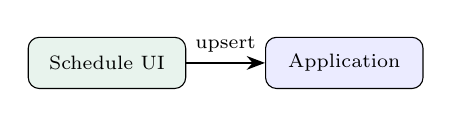
\begin{tikzpicture}[font=\scriptsize, box/.style={draw, rounded corners, align=center, minimum width=2.0cm, minimum height=0.65cm}, arr/.style={-{Stealth}, thick}]
\node[box, fill=leafgreen!12] (s) {Schedule UI};
\node[box, right=1.0cm of s, fill=blue!8] (api) {Application};
\draw[arr] (s) -- node[above] {upsert} (api);
\end{tikzpicture}
\caption{Schedule subsystem persists policies via application APIs.}
\label{fig:pres-sch}
\end{figure}

\subsubsection{Assumptions}
\begin{itemize}
  \item Schedules are stored in a timezone-aware or UTC-normalized manner in the data layer.
\end{itemize}

\subsubsection{Responsibilities}
\begin{itemize}
  \item List and edit schedules with clear scope (tray vs.\ mesh).
  \item Support destination \texttt{raspberry-pi-edge} for edge capture policies.
  \item Validate user inputs (cadence, start/end) before submission.
\end{itemize}

\subsubsection{Subsystem interfaces}
\begin{table}[H]
\centering
\small
\begin{tabular}{|p{0.9cm}|p{3.4cm}|p{3.0cm}|p{3.5cm}|}
\hline
\textbf{ID} & \textbf{Description} & \textbf{Inputs} & \textbf{Outputs} \\
\hline
P-S1 & Schedule UI $\rightarrow$ Application & Schedule DTO & Persisted schedule \\
\hline
\end{tabular}
\caption{Schedule management subsystem interfaces}
\end{table}

\subsection{Devices UI subsystem}

The \textbf{Devices} navigation lists provisioned Raspberry~Pi edge devices for the signed-in owner: CPU serial, online/offline status, last heartbeat, and linked tray. It is the fleet-level companion to the per-tray Raspberry~Pi panel.

\begin{figure}[H]
\centering
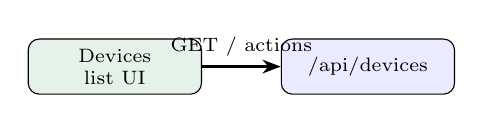
\begin{tikzpicture}[font=\scriptsize, box/.style={draw, rounded corners, align=center, minimum width=2.2cm, minimum height=0.7cm}, arr/.style={-{Stealth}, thick}]
\node[box, fill=leafgreen!14] (dev) {Devices\\list UI};
\node[box, right=1.0cm of dev, fill=blue!8] (api) {/api/devices};
\draw[arr] (dev) -- node[above] {GET / actions} (api);
\end{tikzpicture}
\caption{Devices UI: operator fleet view over edge device APIs.}
\label{fig:pres-devices}
\end{figure}

\subsubsection{Assumptions}
\begin{itemize}
  \item Only devices owned by the authenticated account are visible.
  \item Heartbeat stale windows determine online presentation.
\end{itemize}

\subsubsection{Responsibilities}
\begin{itemize}
  \item Render device inventory and status.
  \item Navigate to linked trays when present.
  \item Surface revoke / rotate-key actions when exposed by product policy.
\end{itemize}

\subsubsection{Subsystem interfaces}
\begin{table}[H]
\centering
\small
\begin{tabular}{|p{0.9cm}|p{3.4cm}|p{3.0cm}|p{3.5cm}|}
\hline
\textbf{ID} & \textbf{Description} & \textbf{Inputs} & \textbf{Outputs} \\
\hline
P-DV1 & Devices UI $\rightarrow$ Application & Session context & Device list DTO \\
\hline
P-DV2 & Devices UI $\rightarrow$ Application & Device action payload & Updated device state \\
\hline
\end{tabular}
\caption{Devices UI subsystem interfaces}
\end{table}

\subsection{Tray Raspberry Pi panel and Take Picture subsystem}

The \textbf{tray Raspberry~Pi panel} embeds edge controls on tray detail: link/unlink device, edit and save \textbf{Klipper/streamer URL} (\texttt{klipper\_url}), generate poses from plant layout, and \textbf{Take Picture}. Take Picture posts \texttt{action=capture} to \texttt{/api/devices/\{id\}}; the UI primarily expects a queued-command acknowledgment for agent \texttt{fswebcam} capture, or an immediate image URL when an optional HTTP streamer is reachable.

\begin{figure}[H]
\centering
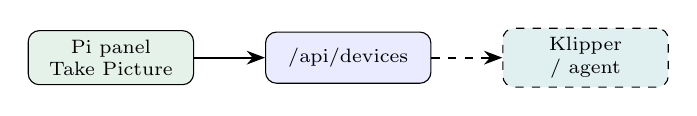
\begin{tikzpicture}[font=\scriptsize, box/.style={draw, rounded corners, align=center, minimum width=2.1cm, minimum height=0.65cm}, arr/.style={-{Stealth}, thick}]
\node[box, fill=leafgreen!14] (panel) {Pi panel\\Take Picture};
\node[box, right=0.9cm of panel, fill=blue!8] (api) {/api/devices};
\node[box, right=0.9cm of api, fill=teal!12, dashed] (hw) {Klipper\\/ agent};
\draw[arr] (panel) -- (api);
\draw[arr, dashed] (api) -- (hw);
\end{tikzpicture}
\caption{Tray Pi panel: Take Picture and Klipper URL management via devices API.}
\label{fig:pres-pi-panel}
\end{figure}

\subsubsection{Assumptions}
\begin{itemize}
  \item Offline empty states are shown when no device is linked or heartbeat is stale.
  \item Klipper/streamer URL updates validate http/https schemes before save.
\end{itemize}

\subsubsection{Responsibilities}
\begin{itemize}
  \item Trigger Take Picture and display returned capture or queue status.
  \item Persist Klipper URL edits (\texttt{updateKlipperUrl}; alias \texttt{updateMoonrakerUrl}).
  \item Support pose generation entry points for multi-angle capture.
\end{itemize}

\subsubsection{Subsystem interfaces}
\begin{table}[H]
\centering
\small
\begin{tabular}{|p{0.9cm}|p{3.4cm}|p{3.0cm}|p{3.5cm}|}
\hline
\textbf{ID} & \textbf{Description} & \textbf{Inputs} & \textbf{Outputs} \\
\hline
P-PI1 & Pi panel $\rightarrow$ Application & \texttt{capture} action & Image URL or queued command \\
\hline
P-PI2 & Pi panel $\rightarrow$ Application & Klipper URL & Updated \texttt{edge\_devices} row \\
\hline
P-PI3 & Pi panel $\rightarrow$ Application & Pose generate request & Pose sequence DTO \\
\hline
\end{tabular}
\caption{Tray Raspberry Pi panel and Take Picture subsystem interfaces}
\end{table}

\newpage

\section{Application Layer Subsystems}
The Application Layer implements the \textbf{control plane} of AgriHome: every client request is authenticated, validated, mapped to domain operations, and translated into data-layer and optional processing-layer calls. Device-key traffic from Raspberry~Pi agents shares the same layer through dedicated \texttt{/api/raspberry-pi/*} routes. The subsystems below follow the decomposition style of the reference architectural document while reflecting AgriHome's agronomic and edge-capture domain.

\subsection{API entry and routing subsystem}

The \textbf{API entry} subsystem exposes HTTP routes and, where used, a GraphQL endpoint. It maps URLs and methods to internal handlers and enforces global concerns such as method allow-lists and body size limits.

\begin{figure}[H]
\centering
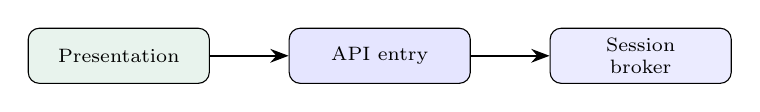
\begin{tikzpicture}[font=\scriptsize, box/.style={draw, rounded corners, align=center, minimum width=2.3cm, minimum height=0.7cm}, arr/.style={-{Stealth}, thick}]
\node[box, fill=leafgreen!12] (cli) {Presentation};
\node[box, right=1.0cm of cli, fill=blue!10] (api) {API entry};
\node[box, right=1.0cm of api, fill=blue!8] (sess) {Session\\broker};
\draw[arr] (cli) -- (api);
\draw[arr] (api) -- (sess);
\end{tikzpicture}
\caption{API entry: first server hop after the presentation layer.}
\label{fig:app-api}
\end{figure}

\subsubsection{Assumptions}
\begin{itemize}
  \item All mutating operator operations require authenticated context unless explicitly public.
  \item Device routes authenticate with provisioning secrets or hashed device API keys rather than Firebase sessions.
  \item Rate limiting may be enforced externally (gateway) or internally per deployment.
\end{itemize}

\subsubsection{Responsibilities}
\begin{itemize}
  \item Accept REST and GraphQL traffic on documented paths, including \texttt{/api/raspberry-pi/*} and \texttt{/api/devices/*}.
  \item Dispatch to validation and domain orchestration pipelines.
  \item Normalize HTTP status codes and error envelopes.
\end{itemize}

\subsubsection{Subsystem interfaces}
\begin{table}[H]
\centering
\small
\begin{tabular}{|p{0.9cm}|p{3.4cm}|p{3.0cm}|p{3.5cm}|}
\hline
\textbf{ID} & \textbf{Description} & \textbf{Inputs} & \textbf{Outputs} \\
\hline
A-R1 & Presentation $\rightarrow$ API entry & HTTP requests & Routed handler \\
\hline
A-R2 & API entry $\rightarrow$ Session broker & Raw request & Auth context \\
\hline
\end{tabular}
\caption{API entry and routing subsystem interfaces}
\end{table}

\subsection{Session and authentication broker subsystem}

This subsystem verifies \textbf{server sessions} established through the identity provider flow, binds the caller to an account key used for data scoping, and rejects stale or forged cookies.

\begin{figure}[H]
\centering
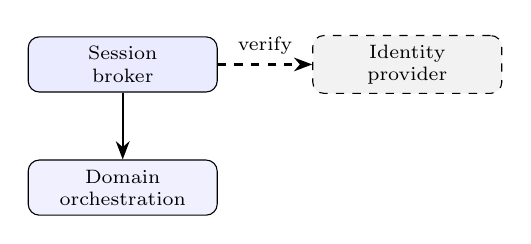
\begin{tikzpicture}[font=\scriptsize, box/.style={draw, rounded corners, align=center, minimum width=2.4cm, minimum height=0.7cm}, arr/.style={-{Stealth}, thick}]
\node[box, fill=blue!8] (sess) {Session\\broker};
\node[box, right=1.2cm of sess, fill=gray!10, dashed] (idp) {Identity\\provider};
\node[box, below=0.85cm of sess, fill=blue!6] (dom) {Domain\\orchestration};
\draw[arr, dashed] (sess) -- node[above] {verify} (idp);
\draw[arr] (sess) -- (dom);
\end{tikzpicture}
\caption{Session broker: establishes trusted account context for downstream work.}
\label{fig:app-session}
\end{figure}

\subsubsection{Assumptions}
\begin{itemize}
  \item Session material is transported only over TLS.
  \item Clock skew between servers remains within acceptable bounds for token validation.
\end{itemize}

\subsubsection{Responsibilities}
\begin{itemize}
  \item Validate session cookies or bearer tokens per integration.
  \item Attach user identity and permissions context to the request scope.
  \item Support sign-out by invalidating server-side session state as implemented.
\end{itemize}

\subsubsection{Subsystem interfaces}
\begin{table}[H]
\centering
\small
\begin{tabular}{|p{0.9cm}|p{3.4cm}|p{3.0cm}|p{3.5cm}|}
\hline
\textbf{ID} & \textbf{Description} & \textbf{Inputs} & \textbf{Outputs} \\
\hline
A-S1 & API entry $\rightarrow$ Session broker & HTTP request & Principal or error \\
\hline
A-S2 & Session broker $\rightarrow$ Domain & Account context & Scoped operations \\
\hline
\end{tabular}
\caption{Session and authentication broker subsystem interfaces}
\end{table}

\subsection{Input validation subsystem}

\textbf{Input validation} enforces structural correctness: JSON schema, multipart boundaries, numeric ranges for schedules, and presence of foreign keys before any database call.

\begin{figure}[H]
\centering
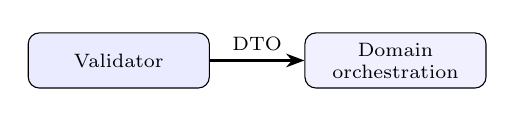
\begin{tikzpicture}[font=\scriptsize, box/.style={draw, rounded corners, align=center, minimum width=2.3cm, minimum height=0.7cm}, arr/.style={-{Stealth}, thick}]
\node[box, fill=blue!8] (v) {Validator};
\node[box, right=1.2cm of v, fill=blue!6] (dom) {Domain\\orchestration};
\draw[arr] (v) -- node[above] {DTO} (dom);
\end{tikzpicture}
\caption{Validation subsystem: rejects bad input early.}
\label{fig:app-val}
\end{figure}

\subsubsection{Assumptions}
\begin{itemize}
  \item All untrusted input arrives through the API entry path.
\end{itemize}

\subsubsection{Responsibilities}
\begin{itemize}
  \item Validate and sanitize payloads; coerce types where safe.
  \item Emit field-level errors consumable by the Presentation Layer.
\end{itemize}

\subsubsection{Subsystem interfaces}
\begin{table}[H]
\centering
\small
\begin{tabular}{|p{0.9cm}|p{3.4cm}|p{3.0cm}|p{3.5cm}|}
\hline
\textbf{ID} & \textbf{Description} & \textbf{Inputs} & \textbf{Outputs} \\
\hline
A-V1 & Session broker $\rightarrow$ Validator & Parsed body & Validated DTO \\
\hline
\end{tabular}
\caption{Input validation subsystem interfaces}
\end{table}

\subsection{Domain orchestration subsystem}

\textbf{Domain orchestration} implements AgriHome use cases: tray and plant CRUD, mesh membership, schedule upserts, monitoring log writes, prediction snapshots, file handoffs, edge device lifecycle, and Take Picture coordination (queued agent \texttt{fswebcam} capture or optional HTTP streamer still). It is the primary caller of the Data Layer and the orchestrator of Processing Layer calls.

\begin{figure}[H]
\centering
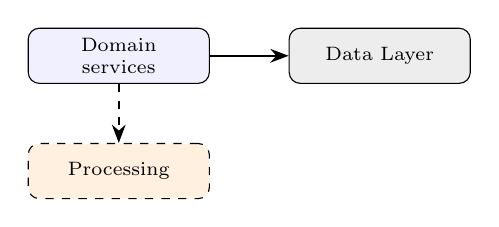
\begin{tikzpicture}[font=\scriptsize, box/.style={draw, rounded corners, align=center, minimum width=2.3cm, minimum height=0.7cm}, arr/.style={-{Stealth}, thick}]
\node[box, fill=blue!6] (dom) {Domain\\services};
\node[box, right=1.0cm of dom, fill=gray!14] (data) {Data Layer};
\node[box, below=0.75cm of dom, fill=orange!12, dashed] (proc) {Processing};
\draw[arr] (dom) -- (data);
\draw[arr, dashed] (dom) -- (proc);
\end{tikzpicture}
\caption{Domain orchestration: central business logic and integration point.}
\label{fig:app-dom}
\end{figure}

\subsubsection{Assumptions}
\begin{itemize}
  \item Domain rules may evolve faster than schema; feature flags may gate behavior.
\end{itemize}

\subsubsection{Responsibilities}
\begin{itemize}
  \item Implement transactional stories that satisfy SRS capabilities.
  \item Map database rows to API DTOs and GraphQL types.
  \item Coordinate retries or compensations when external services fail.
\end{itemize}

\subsubsection{Subsystem interfaces}
\begin{table}[H]
\centering
\small
\begin{tabular}{|p{0.9cm}|p{3.4cm}|p{3.0cm}|p{3.5cm}|}
\hline
\textbf{ID} & \textbf{Description} & \textbf{Inputs} & \textbf{Outputs} \\
\hline
A-D1 & Validator $\rightarrow$ Domain & Valid DTOs & Side effects / results \\
\hline
A-D2 & Domain $\rightarrow$ Data Layer & SQL / storage ops & Persisted state \\
\hline
A-D3 & Domain $\rightarrow$ Processing & Images / metadata & Inference DTOs \\
\hline
\end{tabular}
\caption{Domain orchestration subsystem interfaces}
\end{table}

\subsection{GraphQL query and mutation facade subsystem}

Where enabled, \textbf{GraphQL} provides a typed alternative surface for reads and selected mutations (for example mesh creation, plant updates, schedule upserts). Resolvers delegate to the same domain orchestration as REST to avoid divergent business rules.

\begin{figure}[H]
\centering
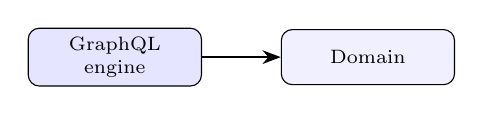
\begin{tikzpicture}[font=\scriptsize, box/.style={draw, rounded corners, align=center, minimum width=2.2cm, minimum height=0.7cm}, arr/.style={-{Stealth}, thick}]
\node[box, fill=blue!10] (gql) {GraphQL\\engine};
\node[box, right=1.0cm of gql, fill=blue!6] (dom) {Domain};
\draw[arr] (gql) -- (dom);
\end{tikzpicture}
\caption{GraphQL facade: thin mapping to domain services.}
\label{fig:app-gql}
\end{figure}

\subsubsection{Assumptions}
\begin{itemize}
  \item GraphQL complexity limits protect against abusive queries.
\end{itemize}

\subsubsection{Responsibilities}
\begin{itemize}
  \item Parse, validate, and execute schema operations.
  \item Return typed errors suitable for client debugging.
\end{itemize}

\subsubsection{Subsystem interfaces}
\begin{table}[H]
\centering
\small
\begin{tabular}{|p{0.9cm}|p{3.4cm}|p{3.0cm}|p{3.5cm}|}
\hline
\textbf{ID} & \textbf{Description} & \textbf{Inputs} & \textbf{Outputs} \\
\hline
A-G1 & Presentation $\rightarrow$ GraphQL & Query/mutation & JSON result \\
\hline
A-G2 & GraphQL $\rightarrow$ Domain & Resolver args & Domain outcomes \\
\hline
\end{tabular}
\caption{GraphQL facade subsystem interfaces}
\end{table}

\subsection{Response and error handling subsystem}

The \textbf{response handler} assembles payloads, sets cache headers where safe, logs structured errors, and ensures that sensitive internals are not leaked to clients—supporting SRS \textbf{security} themes at the API boundary.

\begin{figure}[H]
\centering
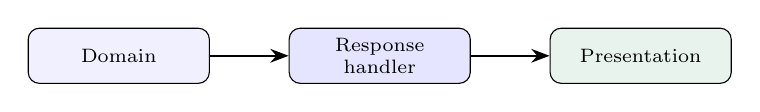
\begin{tikzpicture}[font=\scriptsize, box/.style={draw, rounded corners, align=center, minimum width=2.3cm, minimum height=0.7cm}, arr/.style={-{Stealth}, thick}]
\node[box, fill=blue!6] (dom) {Domain};
\node[box, right=1.0cm of dom, fill=blue!10] (resp) {Response\\handler};
\node[box, right=1.0cm of resp, fill=leafgreen!12] (cli) {Presentation};
\draw[arr] (dom) -- (resp);
\draw[arr] (resp) -- (cli);
\end{tikzpicture}
\caption{Response handler: maps internal results to HTTP/GraphQL responses.}
\label{fig:app-resp}
\end{figure}

\subsubsection{Assumptions}
\begin{itemize}
  \item Central logging infrastructure exists in deployment environments.
\end{itemize}

\subsubsection{Responsibilities}
\begin{itemize}
  \item Serialize success and error bodies consistently.
  \item Map domain exceptions to HTTP status codes.
  \item Redact secrets from logs and client messages.
\end{itemize}

\subsubsection{Subsystem interfaces}
\begin{table}[H]
\centering
\small
\begin{tabular}{|p{0.9cm}|p{3.4cm}|p{3.0cm}|p{3.5cm}|}
\hline
\textbf{ID} & \textbf{Description} & \textbf{Inputs} & \textbf{Outputs} \\
\hline
A-E1 & Domain $\rightarrow$ Response handler & Result / exception & Outbound DTO \\
\hline
A-E2 & Response handler $\rightarrow$ Presentation & HTTP response & Rendered UX \\
\hline
\end{tabular}
\caption{Response and error handling subsystem interfaces}
\end{table}

\subsection{Raspberry Pi edge API subsystem}

The \textbf{Raspberry~Pi edge API} (\texttt{/api/raspberry-pi/*}) is the device-facing control and ingest surface. Agents present a provisioning code at register time and thereafter a device API key (\texttt{X-Agrihome-Device-Key}). Routes cover register, heartbeat (claim pending commands), multipart ingest, command listing, active poses, and capture-plan (schedules + poses + limits).

\begin{figure}[H]
\centering
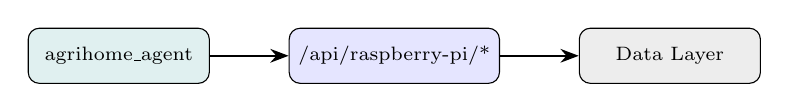
\begin{tikzpicture}[font=\scriptsize, box/.style={draw, rounded corners, align=center, minimum width=2.3cm, minimum height=0.7cm}, arr/.style={-{Stealth}, thick}]
\node[box, fill=teal!12] (agent) {agrihome\_agent};
\node[box, right=1.0cm of agent, fill=blue!10] (rpi) {/api/raspberry-pi/*};
\node[box, right=1.0cm of rpi, fill=gray!14] (data) {Data Layer};
\draw[arr] (agent) -- (rpi);
\draw[arr] (rpi) -- (data);
\end{tikzpicture}
\caption{Raspberry Pi edge API: device-key routes into domain persistence.}
\label{fig:app-rpi}
\end{figure}

\subsubsection{Assumptions}
\begin{itemize}
  \item API keys are stored only as hashes; plaintext is returned once at registration.
  \item Ingest may optionally trigger post-process hooks (plant attach, disease detection).
\end{itemize}

\subsubsection{Responsibilities}
\begin{itemize}
  \item Auto-provision \texttt{edge\_devices} and linked trays on register.
  \item Update online status and claim \texttt{edge\_device\_commands} on heartbeat.
  \item Persist multipart frames to media storage and \texttt{camera\_captures}.
  \item Serve pose sequences and capture plans for multi-angle runs.
\end{itemize}

\subsubsection{Subsystem interfaces}
\begin{table}[H]
\centering
\small
\begin{tabular}{|p{0.9cm}|p{3.4cm}|p{3.0cm}|p{3.5cm}|}
\hline
\textbf{ID} & \textbf{Description} & \textbf{Inputs} & \textbf{Outputs} \\
\hline
A-RP1 & Agent $\rightarrow$ register & Fingerprint + provisioning code & Device/tray IDs + API key \\
\hline
A-RP2 & Agent $\rightarrow$ heartbeat & Device key & Pending commands \\
\hline
A-RP3 & Agent $\rightarrow$ ingest & Multipart image + metadata & Capture DTO / URL \\
\hline
A-RP4 & Agent $\rightarrow$ poses/plan & Device key & Pose sequence / schedule plan \\
\hline
\end{tabular}
\caption{Raspberry Pi edge API subsystem interfaces}
\end{table}

\subsection{Operator devices API subsystem}

The \textbf{operator devices API} (\texttt{/api/devices} and \texttt{/api/devices/\{id\}}) is the session-authenticated control plane for Vision Console operators. It lists devices and performs actions such as \texttt{capture} (Take Picture), \texttt{linkTray}, \texttt{revoke}, \texttt{rotateKey}, and \texttt{updateKlipperUrl} (alias \texttt{updateMoonrakerUrl}). Capture primarily inserts a pending \texttt{capture\_now} for the agent (\texttt{fswebcam}); when \texttt{klipper\_url} is set it may attempt an optional HTTP streamer still first.

\begin{figure}[H]
\centering
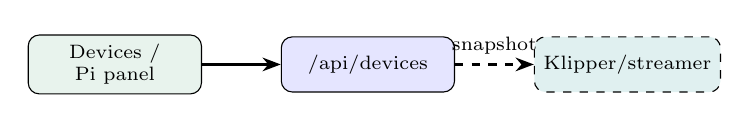
\begin{tikzpicture}[font=\scriptsize, box/.style={draw, rounded corners, align=center, minimum width=2.2cm, minimum height=0.7cm}, arr/.style={-{Stealth}, thick}]
\node[box, fill=leafgreen!12] (ui) {Devices /\\Pi panel};
\node[box, right=1.0cm of ui, fill=blue!10] (dev) {/api/devices};
\node[box, right=1.0cm of dev, fill=teal!12, dashed] (mr) {Klipper/streamer};
\draw[arr] (ui) -- (dev);
\draw[arr, dashed] (dev) -- node[above] {snapshot} (mr);
\end{tikzpicture}
\caption{Operator devices API: Take Picture and device administration.}
\label{fig:app-devices}
\end{figure}

\subsubsection{Assumptions}
\begin{itemize}
  \item Operators may only act on devices they own.
  \item Optional streamer URL candidates include common nginx \texttt{:80} webcam paths derived from \texttt{klipper\_url}.
\end{itemize}

\subsubsection{Responsibilities}
\begin{itemize}
  \item Authorize and execute device actions from the Presentation Layer.
  \item Attempt server-side snapshot before queuing agent capture.
  \item Persist Klipper/streamer URL and linkage changes to \texttt{edge\_devices} / trays.
\end{itemize}

\subsubsection{Subsystem interfaces}
\begin{table}[H]
\centering
\small
\begin{tabular}{|p{0.9cm}|p{3.4cm}|p{3.0cm}|p{3.5cm}|}
\hline
\textbf{ID} & \textbf{Description} & \textbf{Inputs} & \textbf{Outputs} \\
\hline
A-DV1 & Presentation $\rightarrow$ devices API & Session + filters & Device list \\
\hline
A-DV2 & Presentation $\rightarrow$ devices API & \texttt{capture} action & Image URL or queued command \\
\hline
A-DV3 & Presentation $\rightarrow$ devices API & Admin actions & Updated device/tray state \\
\hline
\end{tabular}
\caption{Operator devices API subsystem interfaces}
\end{table}

\newpage

\section{Processing Layer Subsystems}
The Processing Layer encapsulates \textbf{model-based and computer-vision} work for AgriHome, plus \textbf{asynchronous edge capture orchestration}. It is optional in the sense that core monitoring and CRUD remain available without external models; when present, it enriches the product with species hints, tray-level detections, post-ingest disease analysis, and scheduled Pi captures aligned with the SRS's emphasis on plant health insight and automatic image capture.

\subsection{Species and leaf inference adapter subsystem}

This adapter accepts a \textbf{plant or leaf image} (or derived crop) and returns a structured classification: proposed species or cultivar labels, confidence scores, and auxiliary metadata for the Application Layer to store alongside user-confirmed fields.

\begin{figure}[H]
\centering
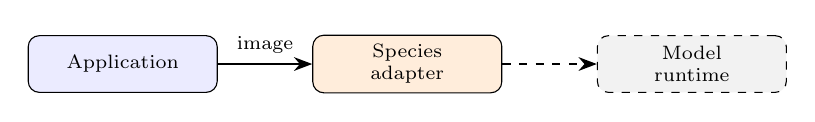
\begin{tikzpicture}[font=\scriptsize, box/.style={draw, rounded corners, align=center, minimum width=2.4cm, minimum height=0.72cm}, arr/.style={-{Stealth}, thick}]
\node[box, fill=blue!8] (app) {Application};
\node[box, right=1.2cm of app, fill=orange!14] (inf) {Species\\adapter};
\node[box, right=1.2cm of inf, fill=gray!10, dashed] (gpu) {Model\\runtime};
\draw[arr] (app) -- node[above] {image} (inf);
\draw[arr, dashed] (inf) -- (gpu);
\end{tikzpicture}
\caption{Species inference adapter: hosted model runtime may be external.}
\label{fig:proc-species}
\end{figure}

\subsubsection{Assumptions}
\begin{itemize}
  \item Network latency between application and adapter is acceptable for interactive flows or runs asynchronously.
  \item Model versioning is tracked so historical reports can be interpreted correctly.
\end{itemize}

\subsubsection{Responsibilities}
\begin{itemize}
  \item Accept a well-defined inference request contract (image bytes or URL, optional tray/plant IDs).
  \item Run the trained classifier or delegate to a managed inference endpoint.
  \item Return normalized labels and scores without persisting domain state itself.
\end{itemize}

\subsubsection{Subsystem interfaces}
\begin{table}[H]
\centering
\small
\begin{tabular}{|p{0.9cm}|p{3.4cm}|p{3.0cm}|p{3.5cm}|}
\hline
\textbf{ID} & \textbf{Description} & \textbf{Inputs} & \textbf{Outputs} \\
\hline
PR-S1 & Application $\rightarrow$ Species adapter & Image + context & Label JSON \\
\hline
PR-S2 & Species adapter $\rightarrow$ Application & HTTP response & Parsed DTO \\
\hline
\end{tabular}
\caption{Species and leaf inference adapter interfaces}
\end{table}

\subsection{Tray vision and layout adapter subsystem}

The \textbf{tray vision} adapter analyzes a tray-level photograph to estimate plant count, regions of interest, or other layout features needed for monitoring dashboards. Outputs are merged into tray records or ephemeral UI state per product rules.

\begin{figure}[H]
\centering
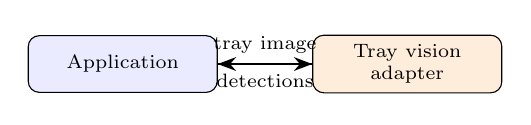
\begin{tikzpicture}[font=\scriptsize, box/.style={draw, rounded corners, align=center, minimum width=2.4cm, minimum height=0.72cm}, arr/.style={-{Stealth}, thick}]
\node[box, fill=blue!8] (app) {Application};
\node[box, right=1.2cm of app, fill=orange!14] (tr) {Tray vision\\adapter};
\draw[arr] (app) -- node[above] {tray image} (tr);
\draw[arr] (tr) -- node[below] {detections} (app);
\end{tikzpicture}
\caption{Tray vision adapter: round-trip inference for tray imagery.}
\label{fig:proc-tray}
\end{figure}

\subsubsection{Assumptions}
\begin{itemize}
  \item Images meet minimum resolution and lighting heuristics expected by the model.
  \item A simulator or stub may substitute in development environments.
\end{itemize}

\subsubsection{Responsibilities}
\begin{itemize}
  \item Detect plants or regions; return geometry in a coordinate system agreed with the UI.
  \item Report confidence and failure modes explicitly.
\end{itemize}

\subsubsection{Subsystem interfaces}
\begin{table}[H]
\centering
\small
\begin{tabular}{|p{0.9cm}|p{3.4cm}|p{3.0cm}|p{3.5cm}|}
\hline
\textbf{ID} & \textbf{Description} & \textbf{Inputs} & \textbf{Outputs} \\
\hline
PR-T1 & Application $\rightarrow$ Tray adapter & Tray image & Detection set \\
\hline
\end{tabular}
\caption{Tray vision and layout adapter interfaces}
\end{table}

\subsection{Inference normalization subsystem}

\textbf{Normalization} converts heterogeneous model outputs into a single internal schema (units, label vocabularies, bounding-box ordering) so the Application Layer can persist results without adapter-specific branches scattered through domain code.

\begin{figure}[H]
\centering
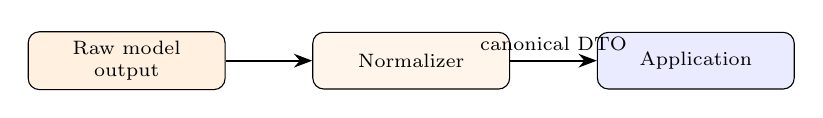
\begin{tikzpicture}[font=\scriptsize, box/.style={draw, rounded corners, align=center, minimum width=2.5cm, minimum height=0.72cm}, arr/.style={-{Stealth}, thick}]
\node[box, fill=orange!12] (raw) {Raw model\\output};
\node[box, right=1.1cm of raw, fill=orange!8] (norm) {Normalizer};
\node[box, right=1.1cm of norm, fill=blue!8] (app) {Application};
\draw[arr] (raw) -- (norm);
\draw[arr] (norm) -- node[above] {canonical DTO} (app);
\end{tikzpicture}
\caption{Normalization: single canonical shape for downstream persistence.}
\label{fig:proc-norm}
\end{figure}

\subsubsection{Assumptions}
\begin{itemize}
  \item Each adapter documents its native schema version.
\end{itemize}

\subsubsection{Responsibilities}
\begin{itemize}
  \item Map labels to controlled vocabularies where required.
  \item Clamp or filter low-confidence results per policy.
  \item Provide stable fields for database columns and UI rendering.
\end{itemize}

\subsubsection{Subsystem interfaces}
\begin{table}[H]
\centering
\small
\begin{tabular}{|p{0.9cm}|p{3.4cm}|p{3.0cm}|p{3.5cm}|}
\hline
\textbf{ID} & \textbf{Description} & \textbf{Inputs} & \textbf{Outputs} \\
\hline
PR-N1 & Adapter $\rightarrow$ Normalizer & Vendor JSON & Canonical inference DTO \\
\hline
PR-N2 & Normalizer $\rightarrow$ Application & Canonical DTO & Ready for persist \\
\hline
\end{tabular}
\caption{Inference normalization subsystem interfaces}
\end{table}

\subsection{Edge disease hook subsystem}

The \textbf{edge disease hook} (\texttt{edge-disease-hook}) runs after a successful Pi ingest or direct capture when a plant ID is present and species inference is configured. It invokes the leaf/species adapter on the stored frame, writes prediction/report outcomes through domain services, and records monitoring events on skip or failure---without failing the ingest itself.

\begin{figure}[H]
\centering
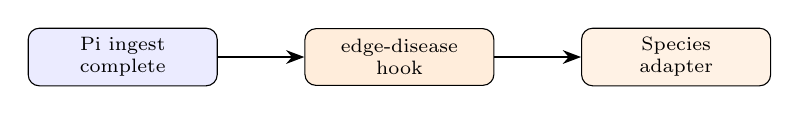
\begin{tikzpicture}[font=\scriptsize, box/.style={draw, rounded corners, align=center, minimum width=2.4cm, minimum height=0.72cm}, arr/.style={-{Stealth}, thick}]
\node[box, fill=blue!8] (ingest) {Pi ingest\\complete};
\node[box, right=1.1cm of ingest, fill=orange!14] (hook) {edge-disease\\hook};
\node[box, right=1.1cm of hook, fill=orange!10] (cv) {Species\\adapter};
\draw[arr] (ingest) -- (hook);
\draw[arr] (hook) -- (cv);
\end{tikzpicture}
\caption{Edge disease hook: optional classification after Pi capture.}
\label{fig:proc-edge-disease}
\end{figure}

\subsubsection{Assumptions}
\begin{itemize}
  \item \texttt{CV\_SPECIES\_INFERENCE\_URL} (or equivalent) may be unset; then the hook records a skip event.
  \item Hook execution is fire-and-forget relative to the HTTP ingest response path when configured asynchronously.
\end{itemize}

\subsubsection{Responsibilities}
\begin{itemize}
  \item Load capture bytes and call plant analysis services.
  \item Persist prediction/report results when inference succeeds.
  \item Emit monitoring events for skip, success, and failure cases.
\end{itemize}

\subsubsection{Subsystem interfaces}
\begin{table}[H]
\centering
\small
\begin{tabular}{|p{0.9cm}|p{3.4cm}|p{3.0cm}|p{3.5cm}|}
\hline
\textbf{ID} & \textbf{Description} & \textbf{Inputs} & \textbf{Outputs} \\
\hline
PR-E1 & Ingest path $\rightarrow$ Edge disease hook & Capture + plant context & Monitoring / prediction side effects \\
\hline
PR-E2 & Edge disease hook $\rightarrow$ Species adapter & Image bytes & Diagnosis DTO \\
\hline
\end{tabular}
\caption{Edge disease hook subsystem interfaces}
\end{table}

\subsection{Capture schedule runner subsystem}

The \textbf{capture schedule runner} (\texttt{capture:schedule-runner}) is a periodic job that evaluates due \texttt{capture\_schedules}. For destination \texttt{raspberry-pi-edge}, it enqueues \texttt{capture\_now} commands (optionally with \texttt{runPoses: true}) onto linked devices so \texttt{agrihome\_agent} performs multi-angle capture without an operator present.

\begin{figure}[H]
\centering
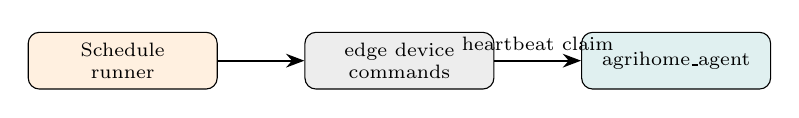
\begin{tikzpicture}[font=\scriptsize, box/.style={draw, rounded corners, align=center, minimum width=2.4cm, minimum height=0.72cm}, arr/.style={-{Stealth}, thick}]
\node[box, fill=orange!12] (runner) {Schedule\\runner};
\node[box, right=1.1cm of runner, fill=gray!14] (cmd) {edge device\\commands};
\node[box, right=1.1cm of cmd, fill=teal!12] (agent) {agrihome\_agent};
\draw[arr] (runner) -- (cmd);
\draw[arr] (cmd) -- node[above] {heartbeat claim} (agent);
\end{tikzpicture}
\caption{Capture schedule runner: enqueues edge capture work for agents.}
\label{fig:proc-sched-runner}
\end{figure}

\subsubsection{Assumptions}
\begin{itemize}
  \item The runner is invoked on a cron-like cadence (for example every minute).
  \item Schedules and device linkage are authoritative in the Data Layer.
\end{itemize}

\subsubsection{Responsibilities}
\begin{itemize}
  \item Select due schedules with edge destinations.
  \item Insert pending capture commands with pose-run flags as configured.
  \item Avoid blocking the interactive Application Layer request path.
\end{itemize}

\subsubsection{Subsystem interfaces}
\begin{table}[H]
\centering
\small
\begin{tabular}{|p{0.9cm}|p{3.4cm}|p{3.0cm}|p{3.5cm}|}
\hline
\textbf{ID} & \textbf{Description} & \textbf{Inputs} & \textbf{Outputs} \\
\hline
PR-R1 & Runner $\rightarrow$ Data Layer & Due schedule query & Schedule/device rows \\
\hline
PR-R2 & Runner $\rightarrow$ Data Layer & \texttt{capture\_now} intents & Pending commands \\
\hline
\end{tabular}
\caption{Capture schedule runner subsystem interfaces}
\end{table}

\newpage

% thebibliography already emits \section*{\refname}; do not add a second References heading
\phantomsection
\addcontentsline{toc}{section}{References}
\begin{thebibliography}{9}
\bibitem{srs}
Agrihome. \textit{System Requirements Specification} (CSE 4316, Spring 2026). Companion requirements document.

\bibitem{nextjs}
Vercel, Inc. ``Next.js Documentation.'' \url{https://nextjs.org/docs} (accessed 2026).

\bibitem{postgres}
PostgreSQL Global Development Group. ``PostgreSQL Documentation.'' \url{https://www.postgresql.org/docs/} (accessed 2026).

\bibitem{firebase}
Google. ``Firebase Authentication.'' \url{https://firebase.google.com/docs/auth} (accessed 2026).

\bibitem{pwa}
W3C. ``Progressive Web Apps.'' \url{https://www.w3.org/TR/appmanifest/} (accessed 2026).
\end{thebibliography}

\end{document}
